\documentclass[a4paper,11pt]{article}
\usepackage[T1]{fontenc}
\usepackage{inputenc}
\usepackage{amsfonts}
\usepackage{graphicx}
\usepackage{bm}
\usepackage{varioref}
\usepackage[english]{babel}
\usepackage{hyperref}
\usepackage{tikz}
\newcommand{\field} [1] {\mathbb{#1}}
\begin{document}

\begin{titlepage}
\centering \parindent=0pt
\newcommand{\HRule}{\rule{\textwidth}{1mm}}
\vspace*{\stretch{1}} \HRule\\[1cm]\Huge\bfseries
Krak-vejkort\\[0.7cm]
\large Visualiseringen\\[1cm]
\HRule\\[4cm]  \large af \\Jacob Stenum Czepluch (jstc@itu.dk), \\Niels Liljedahl Christensen (nlch@itu.dk), \\Mikkel Larsen (milar@itu.dk), \\Sigurt Bladt Dinesen (sidi@itu.dk) \\
\vspace*{\stretch{2}} \normalsize %
\begin{flushleft}
IT-University\\
Copenhagen\\
First year project\\
Rasmus Pagh\\
\today \end{flushleft}
\end{titlepage}

\tableofcontents
\pagebreak

\pagebreak
\section{Introduction}

This will be our introduction to this small report\ldots

We should remember to have a quick bit about how the visualisation works at the moment. The touchpad zoom, mouse move around, and the relative to
mouse pointer placement zoom.

This is a section. Use it. Love it.
This is an example of a long text
This is an example of a long text
This is an example of a long text
This is an example of a long text
This is an example of a long text
This is an example of a long text
This is an example of a long text

Then we have a new line with indent
This is an example of a long text
This is an example of a long text
This is an example of a long text
This is an example of a long text

\pagebreak
\section{Design choices} % (fold)
\label{sec:Design choices}
In this section we will go through our design choices. We will go through things like design pattern, data structure, and visualisation.
At the same time we will give explanations to our choices.

\subsection{Design Pattern} % (fold)
\label{sub:Design Pattern}
For our overall architectural pattern we have chosen to use the Model, View, Controller(MVC) pattern. We chose to do so, to make sure that we have
a very modular and easy to maintain class structure. Using the MVC pattern results in seperation of the different aspects of our application, while still providing a loose coupling between these elements. During this first visualisation part of the application it has proven very useful to us, since we
have been chancing our classes and data structures quite a few times.

% subsection Design Pattern (end)

\subsection{Data Structure} % (fold)
\label{sub:Data Structure}
We started out making a simple data structure that put all the edges into one big ArrayList. This was not fast, but we chose to do it, to make sure that
things were working before we tried implementing a more complicated, but faster data structure. We had several data structures up for discusssion, but we ended up using a quad tree. We actually started out making a kd-tree, but since we had some trouble implmenting it correctly, we decided to take a look
the quad tree aswell. Luckily it turned out to perform very well, and we did not even have to sort our input for it to work well. In our discussion 
section we will further discuss pros and cons of the different data structures.
% subsection Data Structure (end)

\subsection{Visualisation} % (fold)
\label{sub:Visualisation}

% subsection Visualisation (end)

\subsubsection{Platform} % (fold)
\label{subsub:Platform}
To start with we had to decided whether we wanted to use Java and Swing or Java, JavaScript, SVG, and HTML for the visualisation part. There we good and bad things about both. The good thing about Swing was that we all knew how to use it, and we were sure that we were able to do what we wanted in Swing.
%rethink the next bit about good and bad things.
The "bad" thing about Swing is that it does not have as many possibilities as HTML with JavaScript and SVG. The good thing about HTML with JavaScript and SVG would be that it is very easy to customize to look nice and sleek. However, none of us have ever used it before, and since we would rather spend time making something that work and has a nice data structure, we chose to go with Java and Swing.
% subsubsection Platform (end)

\subsubsection{How everything is drawn} % (fold)
\label{subsub:How everything is drawn}
As mentioned above we chose to use Swing and the BasicStroke API to do the drawing of the map. 

Technically the map first draws all of Denmark. It is however only the two biggest road types that are drawn. We decided to do so, because it is both unnessesary to draw all roads, when you are very far away from the map, but also to make the program run smoother. The program is designed to show more and more road types the more you zoom in towards the map. It is only the roads that are inside the given view that are drawn. We have however made a "buffer" that finds the longest road in the view, and extends the frame outside the view with the given lengt. This is done to make sure that all roads are in the view are drawn and vissible.
% subsubsection How everything is drawn (end)

\subsubsection{User interaction} % (fold)
\label{subsub:User interaction}
We wanted to make a very simple yet featurefull user interaction. This resulted in a user interface with no physical buttons. All you need to navigate the map is a mouse. To zoom in and out you either scroll up or down. The mouse pointer decides what the zooming point is. It is also very easy to go up and down or from side to side. This is done my simply dragging and dropping the map with the mouse pointer. Our main reason for making the user interaction like this, is that this way is basically the most intuitive way for a lot of people to navigate and interact with maps and alike, due to the great amount of tablets and smartphones.
% subsubsection User interaction (end)

\pagebreak
\section{Implementation} % (fold)
\label{sec:Implementation} % This sections should describe our implementation
The implementation of the application consists of four different packages; the \texttt{Model}, \texttt{View} and \texttt{Controller} packages used as in the MVC design pattern, and a \texttt{Global} package storing global fields to be accessed and modified from all other packages.


\subsection{Controller package} % This is a simple description of the implementation of the Controller class.
The \texttt{Controller} package consists solely of the \texttt{Controller} class, which is both the main class (it has the main method run when the application starts), and it is the link between the \texttt{Model} and \texttt{View packages} handling the flow of data between the two. When a change is made by the user, the View calls a method in the \texttt{Controller} once again updating the graphical user interface according the both the input from the user and the data stored in the \texttt{Model}.

\subsection{Global package} % Contains all the global values used from all around the application
This package contains only the \texttt{MinAndMaxValues} class which has fields that needs to be accessed from the entire application. These fields include initial values such as the current "viewbox", min and max values for x- and y-coordinates, limits for when the different types of road segments are drawn etc. It also contains methods for checking whether are not the current viewbox results in a need for re-filtering the data to be drawn. The class is statically imported by all classes needing to access this information.

\subsection{Model package} % The description of the Model package is more complicated and consists of descriptions of several other classes.
The \texttt{Model} package consists of all the classes managing data storage, filtering, and conversion.

\subsubsection{Model class} % Makes use of the rest of the classes in the Model package. The front-end class.
The \texttt{Model} class is the front-end class of the \texttt{Model} package (the only class which is directly connected to the \texttt{Controller} class). This is where the data structure is stored in a field and where the methods for filtering and converting data are called. The data structure is stored with the type \texttt{DataStructure}, which is an interface allowing us to easily switch between data structures, as long as they implement this interface.

\subsubsection{XMLReader class} % Reads in the data from an XML file of krax format and adds the content to a given data structure
This class reads in data from an XML file of the KRAX format and converts it to instances of the \texttt{Edge} class (a simple class representing an edge on the roadmap), which then are added to a given data structure.

The \texttt{XMLReader} makes use of an external library, \href{www.xom.nu}{\texttt{xom}} (\url{www.xom.nu}), for reading the XML data.

\subsubsection{QuadTreeDS class} % The data structure of the application. Consists of several other classes to be explained here
The \texttt{QuadTreeDS} is the basis of the entire application. It is in an instance of this all data is stored after being read by the \texttt{XMLReader} class. In order for it to be used as our data structure, it implements the \texttt{DataStructure} interface.

The class consists of four instances of the \texttt{QuadTree} class (one for each type of road segment). A \texttt{QuadTree} consists of nodes, which has an x- and a y-coordinate (stored as \texttt{double}) and a reference to an \texttt{Edge} object. Each \texttt{QuadTree} contains all edges of a given type. Each \texttt{Edge} object is stored twice; both referenced to by the start- and end-coordinates of the edge.

Inserting a node into a \texttt{QuadTree} is done recursively; the given node is compared to root node, deciding to which of the four children of the root the given node is to be compared to next. This continues until a null-reference / a leaf is found.

Retrieving information is done using an instance of the \texttt{Interval2D} class (representing a rectangle), which again consists of to instances of the \texttt{Interval} class (representing a line). This too is done recursively; it is checked whether the coordinates of the root node is within the given rectangle. If it is, it is added to a given collection of edges. It is then checked which of the subtrees might contain nodes within the rectangle, and for each that match, the same method is invoked, now with each of the matching children as the root. The call returns at null references.

Out implementation of the quadtree (including the \texttt{Interval} and \texttt{Interval2D} classes) are heavily based upon implementations from
\url{algs4.cs.princeton.edu}.

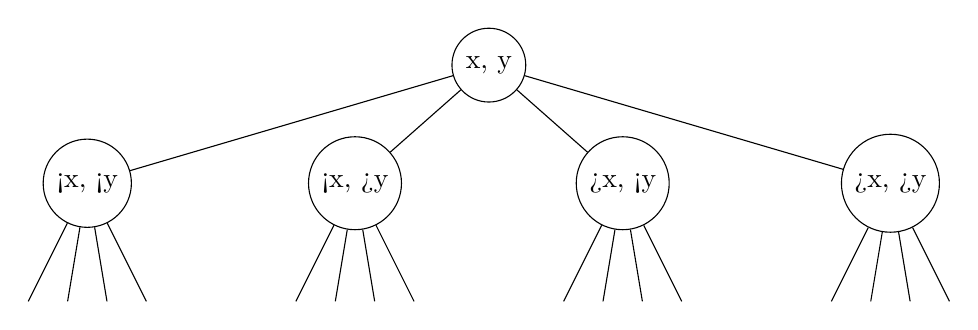
\begin{tikzpicture}
	[level 1/.style={sibling distance=34mm},
	level 2/.style={sibling distance = 5mm}]
	\tikzstyle{every node}=[circle,draw]
	\node {x, y}
		child {
			node {<x, <y}
			child
			child
			child
			child
		}
		child {
			node {<x, >y}
			child
			child
			child
			child		
		}
		child {
			node {>x, <y}
			child
			child
			child
			child		
		}
		child {
			node {>x, >y}
			child
			child
			child
			child		
		}
	;
\end{tikzpicture}

\subsubsection{FormatConverter class} % Converts from the data type pulled out of the data structure to the data type needed by the View package
The \texttt{FormatConverter} has static methods only, and only one public method. This methods takes an \texttt{ArrayList<Edge>} and converts it to the type \texttt{int[][][]} (\texttt{int[type][number of edges][edge coordinates]}).

The FormatConverter uses an instance of the Coordinates class, which converts the given UTM32 coordinates to pixels as shown in the GUI.

\subsubsection{KrakToXMLConverter class} % Not directly part of the implementation, but the class used for converting the data from Krak to the krax XML format
The KrakToXMLConverter is not directly a part of the application (it is not used runtime). It is a util class, reading in the data supplied by Krak, writing it to an XML file of the KRAX format (once again using the external \href{www.xom.nu}{\texttt{xom}} library).

\subsection{View package} % Consists of all the classes handling the graphical user interface
The \texttt{View} package contains all the classes managing the graphical user interface.

\subsubsection{View class} % Front end class in the MVC pattern. Contains the rest of the (non-static) GUI classes. Implements the MapListener interface. The overall class structure of the View package
The \texttt{View} class is the front end class of the \texttt{View} package in the MVC design pattern. It contains an instance of the \texttt{MainFrame} class, which is the basic \texttt{java.swing} GUI (the window to be displayed), which then again contains an instance of our custom panel, \texttt{MapPanel}.

The \texttt{View} itself implements the interface \texttt{ViewListener}, of which an instance is stored in both the \texttt{MainFrame} and the \texttt{MapPanel} classes. This allows for these class to invoke a method in the \texttt{View}, telling it that changes has been made, which then invokes a similar method in the \texttt{Controller}, which then updates the GUI according the the changes.

\subsubsection{MapPanel class} % Draws lines according to input data
The \texttt{MapPanel} class extends the \texttt{java.swing.JPanel} class and cuntions as a panel with added functionality and with an overridden \texttt{paint} method.

The \texttt{MapPanel} stored an \texttt{int[][][]} (as generated by the \texttt{FormatConverter}), from which it it draws lines of the canvas, each corresponding to an edge stored in the \texttt{Model}.

The \texttt{MapPanel} also has to listeners from the \texttt{java.awt} library; a MouseWheelListener, which invokes a static method of the \texttt{ZoomHandler} class when the user scrolls on the panel, sending info about the mouse coordinates and the amount scrolled, and a MouseMotionListener, which invokes a static method of the \texttt{DragHandler} class when the user drags the mouse on the panel, sending info about how far the mouse has been dragged (and along which axes).

\subsubsection{ZoomHandler class} % Handles all the zooming
The \texttt{ZoomHandler} handles all the zooming. When receiving a method call (from the \texttt{MapPanel}) saying that the user tries to zoom out, there are to possible cases; if the current viewbox is not close to the max of the width and height values, it zooms out, keeping the current center of the viewbox the center. Else, zooming is done so  the viewbox follows the borders created by the max values.

Zooming in is followed by a method call on the \texttt{DragHandler} class, moving the viewbox towards the current location of the cursor.

Zooming is simply changing the global values of what is shown (in the \texttt{MinAndMaxValues} class) / changing the size of the viewbox and then invoking a repaint of the \texttt{MapPanel}.

\subsubsection{DragHandler class} % Handles all the dragging
The \texttt{DragHandler} class, like the \texttt{ZoomHandler} class, changes the viewbox according to input data (drag amount and direction) and according the the max values / borders of how far left / right / up / down the viewbox can go.

\pagebreak
\section{Discussion} % (fold)
\label{sec:Discussion}
In this sections we will discuss what could have been done better, and/or what we think we have done right.

\subsection{Outline}
\begin{description}
	\item[Limitations] \hfill \\
	
	\item[Possible improvements] \hfill \\
	
	\item[Data structure discussion] \hfill \\
	QuadTree vs KD-tree
	
	Balanced vs unbalanced QuadTree
\end{description}
% section Discussion (end)

\pagebreak
\section{Conclusion} % (fold)
\label{sec:Conclusion}
This section will make a quick summary and conclusion on out project so far.
% section Conclusion (end)

\subsection{Test 2}

This is a subsection

\end{document}
